%TODO: Need to proof read the math
\section{Scalable Aggregation at a Router's Line Rate}
\label{sec:aggregation}

How should routers implement \TheSystem's language constructs? We require
instructions on routers that can aggregate packets into per-flow state ({\ct
groupby}), transform packet fields ({\ct map}), stream only packets matching a
predicate ({\ct filter}), or merge packets that satisfy two previous queries
({\ct zip}).

Of these four language constructs, three ({\ct map}, {\ct filter}, and {\ct
zip}) are {\em stateless}: they operate on packet fields alone and do not
modify router state. Such stateless manipulations are already supported by
emerging programmable routers that support programmable packet header
processing~\cite{rmt, xpliant, flexpipe, tofino}. On the other hand, the {\ct
groupby} construct needs to maintain and update router state on a per-flow
basis.

%It is the
%most powerful of our language constructs and captures the kind of complex
%processing typically seen at end hosts.

Stateful manipulation on a router for a {\ct groupby} is challenging for two
reasons. First, the time budget to update state before the next packet arrives
at a router can be as low as 1 ns on high speed routers~\cite{domino_sigcomm}.
Second, the router needs to maintain state proportional to the number of
aggregated records (\eg per flow), which may grow unbounded with time. We
address both challenges using a programmable key-value store in hardware. The
keys represent aggregation fields (\eg the five tuple) and the values represent
the state being updated by the aggregation function (\eg a packet or byte
counter). 

However, memories can either be fast and small (SRAM) or slow and large (DRAM),
but not both. Hence, our key-value store has a `split' design.  A small and
fast on-chip key-value store on the router's on-chip SRAM processes packets at
the router's line rate. This on-chip key-value store serves as a cache for a
large and slow off-chip backing store in DRAM that can hold a large number of
flows.

 In traditional cache designs, cache misses require accessing off-chip DRAM
with non-deterministic latencies~\cite{unpredictable_cache} to read out the
stored state. Because the aggregation operation requires us to read the value
in order to update it, the entire state update operation incurs
non-deterministic latencies in the process.  This results in stalls in the
router pipeline. Unfortunately, pipeline stalls affect the ability to provide
guarantees on line-rate packet processing (10--100 Gbit/s) on all router ports.

\begin{figure}
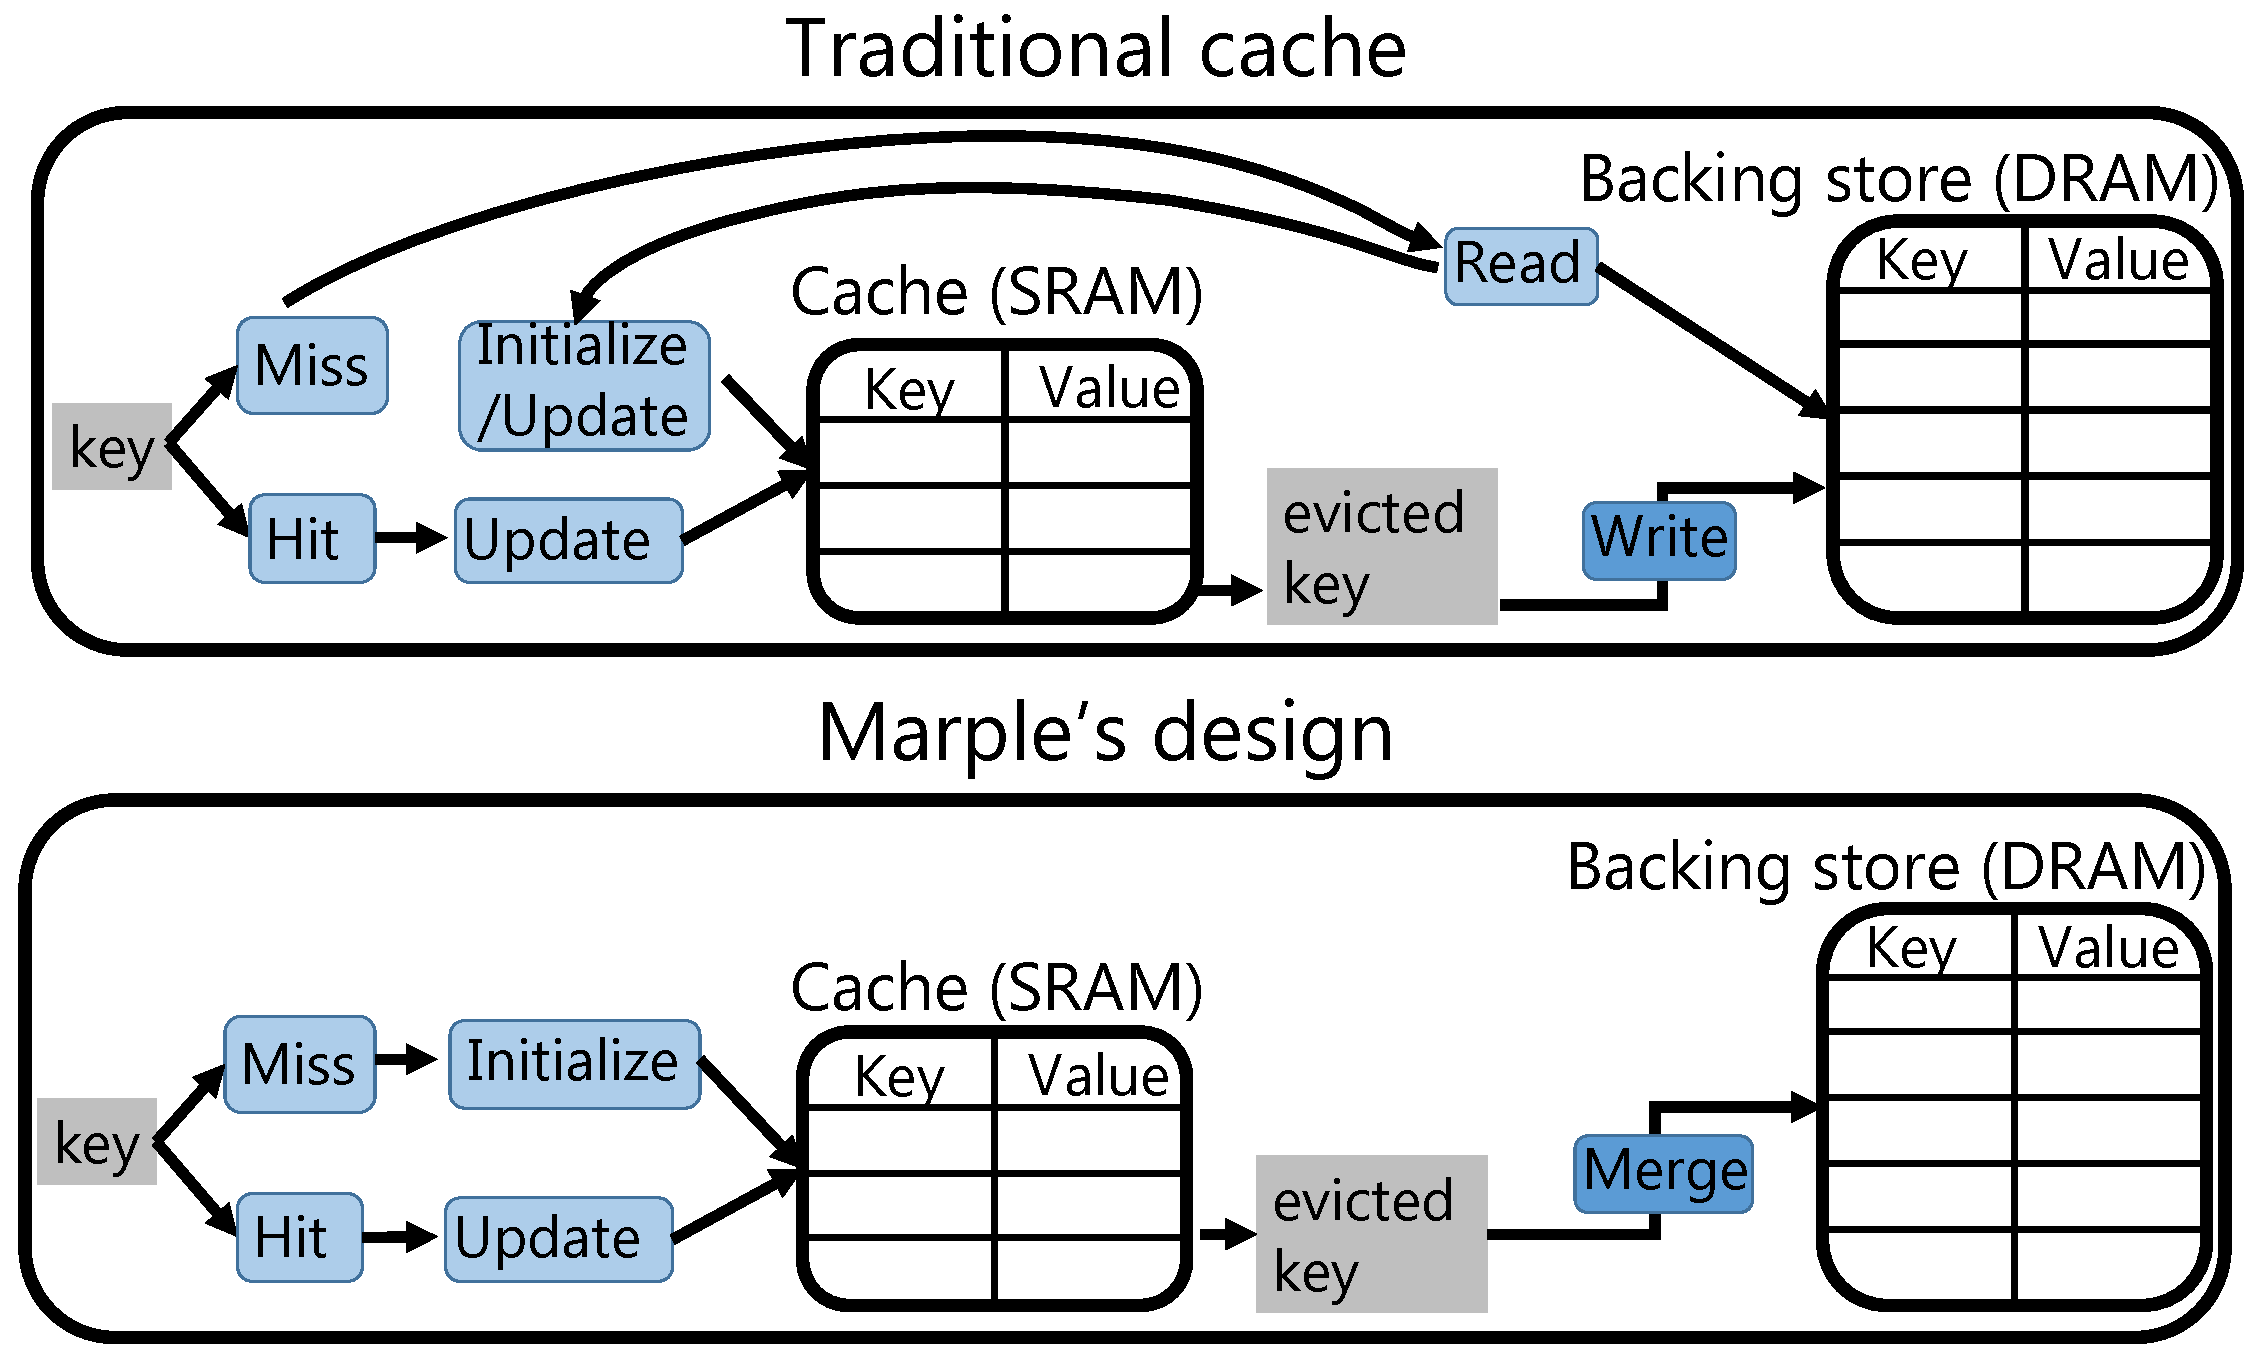
\includegraphics[width=\columnwidth]{pq_kv_store.pdf}
\caption{\TheSystem's key-value store vs. a traditional cache}
\label{fig:kv}
\end{figure}

To avoid such non-determinism, we design our key-value store to process packets
at the router's line rate even on cache misses (Figure~\ref{fig:kv}). Instead
of stalling the pipeline waiting for a result from DRAM, we treat the incoming
packet as the first packet from a new flow and initialize the flow's state to
an initial value.  Subsequent packets from the same flow are aggregated within
the newly created flow entry in the key-value store, until the flow is evicted.
When the flow is eventually evicted, we merge the flow's value just before
eviction with its value in the backing-store using a {\em merge function}, and
write the merged result to the backing store.

In our design, the router only writes to the backing store during evictions,
which is off the critical path of packet processing. Importantly, it never
reads from the backing store during cache misses, which is on the critical path
of packet processing. This helps us avoid non-deterministic latencies.  The
backing store may be stale relative to the on-chip cache if there have been no
recent evictions. We remedy this by forcing periodic evictions.

To merge a flow's new aggregated value in the cache with its old value in the
backing store, the cache needs to maintain and send {\em auxiliary state} to
the backing store during evictions.  A \naive usage of auxiliary state is to
store relevant fields from every packet of a flow, so that the backing store
can simply run the aggregation function over all the newly received packets when
merging.  However, in a practical implementation, the auxiliary state should be
bounded in size and not grow with the number of packets in the flow.

Over the next four subsections, we describe two classes of queries that are
{\em mergeable} with a small amount of auxiliary state (\S\ref{sec:associative}
and \S\ref{sec:linear-in-state-description}), discuss queries that are not
mergeable (\S\ref{sec:workaround-nonscalable}), and provide a general condition
for mergeability that unifies the two classes of mergeable queries and
separates them from non-mergeable queries (\S\ref{sec:unifies}).
%TODO: Consider adding Amy's Venn diagram

\subsection{The associative condition}
\label{sec:associative}

A simple class of mergeable aggregations is the class of associative functions.
Suppose the aggregation function on state $s$ is $s = op(s, f)$, where $op$ is
an associative operation and $f$ is a packet field. Then, if $op$ has an
identity element $I$\footnote{An identity element $I$ for an operation $op$ is
an element such that $op(s, I) = s \forall s$.} and a flow's default value on
insertion is $s_0 = I$, it is easy to show that this function can be merged
using the function $op(s_{backing}, \scache)$, where $s_{backing}$ and
$\scache$ are the value in the backing store and the value just evicted from
the cache, respectively. The associative condition allows us to merge
aggregation functions like addition, max, min, set union, and set intersection.

% resume at assoc condition
\subsection{The linear-in-state condition}
\label{sec:linear-in-state-description}

Consider the EWMA aggregation function, which maintains a moving
average of queueing latencies across all packets within a flow. The aggregation
function updates the EWMA $s$ as follows:
\[ s = (1 - \alpha) \cdot s + \alpha \cdot (t_{out} - t_{in}) \]
We initialize $s$ to $s_0$. Suppose a flow $F$
is evicted from the on-chip cache for the first time and written to the backing
store with an EWMA of $s_{backing}$.\footnote{When a flow is first evicted, it does
not need to be merged.} The first packet from $F$ after $F$'s eviction is
processed like a packet from a new flow in the on-chip cache, starting with the
state $s_0$. Assume that $N$ packets from $F$ then hit the on-chip cache,
resulting in the EWMA going from $s_0$ to $\scache$.
Then, the correct EWMA $s_{correct}$ (\ie for all packets seen up to this point) satisfies:
\begin{align*}
s_{correct} - (1-\alpha)^N s_{backing} &= \scache - (1-\alpha)^N s_0 \\
s_{correct} &= \scache + (1-\alpha)^N(s_{backing} - s_0)
\end{align*}
So, the correct EWMA can be obtained by: (1) having the on-chip cache store
$(1-\alpha)^N$ as auxiliary state for each flow after each update, and
(2) adding $(1-\alpha)^N(s_{backing} - s_0)$ to $\scache$ when merging
$\scache$ with $s_{backing}$.

We can generalize this example. Let $\mathbf{p}$ be a
vector with the headers and performance metadata from the last $k$
packets of a flow, where $k$ is an integer determined at query
compile time (\S\ref{sec:linear-in-state-compilation}).
We can merge any aggregation function with state updates of the form
$\boldsymbol{S} = \boldsymbol{A}(\mathbf{p}) \cdot
\boldsymbol{S} + \boldsymbol{B}(\mathbf{p})$, where
$\boldsymbol{S}$ is the state, and
$\boldsymbol{A}(\mathbf{p})$ and $\boldsymbol{B}(\mathbf{p})$ are
functions of the last $k$ packets. We call this condition the
{\em linear-in-state} condition and say that $\boldsymbol{A}(\mathbf{p})$
and $\boldsymbol{B}(\mathbf{p})$ are functions of {\em
bounded packet history.}

The requirement of bounded packet history is important.
Consider the TCP non-monotonic query from \Fig{example-perf-queries}, which
counts the number of packets with sequence numbers smaller than the maximum
sequence number seen so far. The aggregation can be expressed as
\begin{lstlisting}
count = count + (maxseq > tcpseq) ? 1 : 0
\end{lstlisting}
While the update superficially resembles $\boldsymbol{A}(\mathbf{p}) \cdot \boldsymbol{S} +
\boldsymbol{B}(\mathbf{p})$, the coefficient $\boldsymbol{B}(\mathbf{p})$ is a function of {\ct
maxseq}, the maximum sequence number so far, which could be arbitrarily far
back in the stream.
%
Intuitively, since $\boldsymbol{B}(\mathbf{p})$ is not a function of bounded packet history,
the auxiliary state required to merge {\ct count} is large.
\Sec{unifies} formalizes this intuition.

In contrast, the slightly modified TCP out-of-sequence query from \Fig{example-perf-queries} {\em is}
linear-in-state because it can be written as
\begin{lstlisting}
count = count + (lastseq > tcpseq) ? 1 : 0
\end{lstlisting}
where {\ct lastseq}, the previous packet's sequence number, depends only on the last 2 packets: the current and the previous packet. Here,
$\boldsymbol{A}(\mathbf{p})$ and $\boldsymbol{B}(\mathbf{p})$ are functions of bounded packet history,
with $k = 2$.
%  This is in contrast to {\ct maxseq}, which depends on all packets seen so far.

Merging queries that are linear-in-state requires the router to store
the first $k$ and most recent $k$ packets
for the key since it (re)appeared in the key-value store; details are
available in the appendix (Appendix~\ref{app:merge}).

An aggregation function is linear-in-state
if, for every variable in the function, the state update
satisfies the linear-in-state condition. A query is linear-in-state
if all its aggregation functions are linear-in-state.

\subsection{Scalable aggregation functions}
\label{sec:scalable}
A {\ct groupby} with no {\ct emit()} and a linear-in-state (or associative) aggregation function
can be implemented scalably without losing accuracy. Examples of such
aggregations (from \Fig{example-perf-queries}) include tracking successive
packets within a TCP connection that are out-of-sequence and counting the
number of TCP timeouts per connection.
%

 If a
{\ct groupby} uses an {\ct emit()} to pass tuples to another query, it cannot be
implemented scalably even if its aggregation function is linear-in-state or associative. An {\ct emit()} outputs the current state of the
aggregation function, which assumes the current state is always available in
the router's on-chip cache. This is only possible if flows are never evicted,
effectively shrinking the key-value store to its on-chip cache alone.

\subsection{Handling non-scalable aggregations}
\label{sec:workaround-nonscalable}
While the linear-in-state and associative conditions capture several
aggregation functions and enable a scalable implementation, there are two
practical classes of queries that we cannot scale: (1) queries with aggregation
functions that are neither associative nor linear-in-state and (2) queries where
the groupby has an {\ct emit()} statement.

An example of the first class is the TCP non-monotonic query discussed earlier.
An example of the second class is the flowlet size histogram
query from~\Fig{example-perf-queries}, where the first {\ct groupby} emits
flowlet sizes, which are grouped into buckets by the second {\ct groupby}.

There are workarounds for non-scalable queries. One is to rewrite queries to
remove {\ct emit()}s.  For instance, we can rewrite the loss rate query
(\Fig{example-perf-queries}) to independently record the per-flow counts for
dropped packets and total number of packets in separate key-value stores, and
have an operator consult both key-value stores every time they need the loss
rate. Each key-value store can be scaled, but the implementation comes at a
transient loss of accuracy relative to precisely tracking the loss rate after
every packet using a {\ct zip.} Second, an operator may be content with flow
values that are accurate for each time period between two evictions, but not
across evictions (\Fig{accuracy-time}). Third, an operator may want to run a
query to collect data until the on-chip cache fills up and then stop data
collection.  Finally, if the number of keys is small enough to fit in the cache
(\eg if the key is an application type), the system can provide accurate
results without evicting any keys.

\subsection{A unified condition for mergeability}
\label{sec:unifies}
We present a general condition that separates mergeable functions from
non-mergeable ones.
Informally, mergeable aggregation functions are those that maintain auxiliary state
linear in the size
of the function's state itself.
This characterization also has the benefit of unifying the associative and
linear-in-state conditions.
We now formalize
our results in the form of several theorems.

First, we introduce some formal notation (\S\ref{ss:notation} and \S\ref{ss:closure})
before presenting the theorems (\S\ref{ss:proofs}).

\subsubsection{Notation}
\label{ss:notation}

A programmer supplies an aggregation function $f$. $f$ takes as inputs an n-bit \emph{state}
vector and a p-bit \emph{packet header} vector and returns an updated $n$-bit
\emph{state} vector. $f$ captures incremental computations over packet streams,
such as a count of packets or an exponentially weighted moving average of
packet latencies. $f$ can only represent incremental computations where the
size of state is fixed and doesn't grow with the length of the packet stream.
For example, $f$ can't represent a median over the packet stream.

Given $f$, we want two implementation functions: an incremental function implementation $g$
 and merge function implementation $m$ that can merge results from
running $f$ over separate packet streams. Specifically, can we merge
two results from running $f$ on two packet streams into one result,
equivalent to running $f$ on the concatenated stream? Formally, we suppose that the state used by
the implementation is $n' \geq n$ bits.

\begin{align}
f : \{0, 1\}^n \times \{0, 1\}^p & \rightarrow \{0, 1\}^n \mbox{(programmer's incremental computation)} \nonumber \\
g : \{0, 1\}^{n'} \times \{0, 1\}^p  & \rightarrow \{0, 1\}^{n'} \mbox{(implementation's incremental computation)} \nonumber \\
m : \{0, 1\}^{n'} \times \{0, 1\}^{n'} & \rightarrow \{0, 1\}^{n'} \mbox{(implementation's merge operation)} \nonumber \\
h : \{0, 1\}^{n'}               & \rightarrow \{0, 1\}^n  \mbox{(transform
 implementation state to programmer state)} \nonumber \\
s_0  & \in \{0, 1\}^n \mbox{(programmer's start state)} \nonumber \\
s'_0 & \in \{0, 1\}^{n'} \mbox{(implementation's start state)} \nonumber \\
m(s'_0, s') & = s' \ \ \forall s \in \{0, 1\}^{n} \mbox{($s'_0$ is an identity for $m$)} \nonumber \\
(g, m, h, s'_0) & \mbox { merges } (f, s_0) \mbox{ if} \nonumber \\
s_0 & = h(s'_0) \mbox{(implementation's start matches with programmer's start)} \label{eqn:start_condition} \\
f(f(f(s_0, P_1), P_2), \dots, P_n) & = h(g(g(g(s'_0, P_1), P_2), \dots, P_n)) \ \forall n \in \mathbb{N} \ \ P_1, P_2, \dots, P_n \in \{0, 1\}^p \label{eqn:projection_condition} \\
h(g(g(g(s'_0, P_1), P_2), \dots, P_{i+j})) & =h( m(g(g(g(s'_0, P_1), P_2), \dots, P_{i}), \nonumber \\
&\ \ \ \ g(g(g(s'_0, P_{i+1}), P_{i+2}), \dots, P_{i+j}))) \nonumber \\
\forall i, j \in \mathbb{N} & \ \  P_1, P_2, \dots, P_{i+j} \in \{0, 1\}^p \label{eqn:merge_condition}
\end{align}

%TODO: What does efficiently computable mean? Be precise.
Here $f, g, m,$ and $h$ are assumed to be efficiently computable functions. We use the notation $f(s, \{p_1, \ldots p_k\})$ to denote the composition of $f$ over a sequence
of packets, similar to a fold function. Additionally, we say that a merge function successfully merges an aggregation function if Equation~\ref{eqn:merge_condition} holds. 

%TODO: DO we need to mention this new made-up notation for composition of $f$ over a sequence of packets?

\subsubsection{The closure graph}
\label{ss:closure}

Before proceeding with the proofs, we introduce the directed \emph{closure graph} of $f$, denoted $G(f)$. Suppose that at some point during the aggregation, 
the programmer specified state is $s$. After running through some additional packets, that state is updated to $s'$. If $s$ is known, then computing
$s'$ is straightforward: simply execute the aggregation $f$ on all the packets seen in the interim. However, if $s$ is \emph{not} known, we can instead
use the packets seen to compute a function that tells us how to get from \emph{a symbolic} state $s$ to the final desired state $s'$. That is, given a sequence of packets $\{p_k\}$,
we can compute an \emph{iterated} function $f_i \in \{0,1\}^n \rightarrow \{0,1\}^n$, such that for any state $s$, $f_i(s) = f(s, \{p_k\})$. For an empty sequence, the corresponding iterated function is the identity.
Our goal is to store some compact representation of the iterated function in the on-chip cache as part of the auxiliary state. Conceptually,  this iterated function is updated with each new packet that is seen, so that when a key is evicted from the on-chip cache,
an identifier for the updated iterated function is sent to the backing store. The backing store then applies this iterated function to the state $s_{backing}$ stored from a previous eviction to get the new value.

How does one update the iterated function stored on the router? The vertices of the closure graph of $f$ are iterated functions $f_i$, and we let $|G(f)|$ indicate the number of vertices. Since there are a finite number of functions $\{0, 1\}^n \rightarrow \{0, 1\}^n$, the size of the graph is bounded.
Each vertex has an outgoing edge corresponding to every possible packet. For a given packet $p$, the iterated function $f_i$ has an edge to the function $f_j$ satisfying $f(f_i(s), p) = f_j(s)$ for all $s$.
The closure graph thus has the following property: given a sequence of packets $\{p_1, \ldots p_k\}$, start at the identity function and, on the $i$th step, follow the edge corresponding to each packet $p_i$. The ending vertex of this process is the iterated function that captures the effect of this packet sequence on any starting state. We say that this ending vertex is the result of \emph{updating the iterated function} by the given sequence of packets. To update the iterated function stored on the router given a new packet, simply follow the edge labeled with that packet.

\subsubsection{Proofs of theorems}
\label{ss:proofs}

\begin{theorem}
A merge function exists to successfully merge an aggregation function $f$,
provided it can use up to $n2^n$ auxiliary bits.
\end{theorem}
\begin{proof}
We can represent each iterated function $f_i$ in $n2^n$ bits, using a list of $2^n$ $n-$bit numbers. This list enumerates the output of the iterated function on every possible input, \ie the $k$th item in the list is $f_i(k)$. The router stores this representation. For each new packet $p$, the router computes the update to each number in the list: $f_i(k) \rightarrow f(f_i(k), p)$. Upon a merge, the router sends this representation to the backing store, which can then evaluate $f_i(s_{backing})$, where $s_{backing}$ is the value stored in the backing store.
\end{proof}

Note that the router needs to tell the backing store what update to perform on the value it currently has. Each iterated function in the closure graph is a possible update, so the router needs to convey at least $\log |G(f)|$ auxiliary bits for the merge to be possible.

As an example, consider a simple counter, where $f(s, p) = s + 1$ and $s_0 = 0$. If the counter has $n$ bits, the closure graph is a ring of size $2^n$, where the $i$th vertex represents the iterated function $f_i(s) = s + i$. Note that all edges from the $i$th vertex point to the $i+1$st vertex. For every observed packet, the router walks one step further around the ring. This is implemented efficiently via adding 1 to an $n$-bit counter. After $K$ packets, the iterated function on the router is $f_{k}$, where $k = K \mod 2^n$. Upon merging, this is sent to the backing store, which then knows to add $k$ to the existing backing store value.

In general, requiring $n2^n$ bits is typically infeasible for even moderate values of $n$. This is where the linear-in-state and associative conditions come in. We show that either of these conditions is enough to require only $O(n)$ auxiliary bits of space.

\begin{theorem}
 Aggregation functions that are either linear-in-state or associative have a
merge function that uses only $O(n)$ auxiliary bits.
\end{theorem}
\begin{proof}
The associative condition is trivial: by definition, no auxiliary bits are required because the merge function simply applies the original aggregation function on the values in the cache and the backing store. Hence, we focus on the linear-in-state condition.
Suppose $f$ is an aggregation function that is linear-in-state, \ie $f(\mathbf{S}, p) = \mathbf{A}(p) \cdot \mathbf{S} + \mathbf{B}(p)$, where $\mathbf{S}$ is a state vector, and $\mathbf{A,B}$ are matrices depending only on the incoming packet. Then:
\[ f(\mathbf{S}_0, \{p_1, \ldots, p_k\}) = \mathbf{A}(p_k)\ldots \mathbf{A}(p_1) \cdot \mathbf{S}_0 + \mathbf{C}(p_1, p_2, \ldots, p_k) \equiv \mathbf{A'} \cdot \mathbf{S}_0 + \mathbf{C}(p_1, \ldots, p_k)\]
where $\mathbf{C}$ is some function of only the packets and $\mathbf{A'}$ is a composition of the $\mathbf{A}$ matrices for the observed packets. The router keeps track of $\mathbf{A'}$ and $\mathbf{C}$, which requires $O(nd^2)$ space where $d$ is the number of pieces of state, each of which we assume has size $n$. These matrices are sent to the backing store upon eviction, at which point the merge operation computes the new backing store value:
\[ \mathbf{S}_d \leftarrow \mathbf{C}(p_1, \ldots, p_k) + \mathbf{A'} \cdot \mathbf{S}_d \]
It's easy to verify that this is the proper merge procedure.
\end{proof}
%TODO: extensions to bounded packet history

However, there are some functions that are not mergeable with so few auxiliary bits. Take the following TCP-non-monotonic function:
\begin{verbatim}
def nonmt(maxseq, count, tcpseq):
  if maxseq > tcpseq:
    count = count + 1
  else:
    maxseq = tcpseq
nm_q = groupby(pktstream, 5tuple, nonmt);
\end{verbatim}

\begin{theorem}
The TCP-non-monotonic function requires at least $n2^n$ auxiliary bits to merge.
\end{theorem}
\begin{proof}
Two pieces of state must be stored: the max sequence number and the count. For
simplicity, we assume each piece of state requires $n$ bits.
We present a family of packet sequences, such that there is an injection between the sequences and vertices in the closure graph of $f$. In other words, starting from the identity, updating the identity iterated function by each sequence in this family will result in a distinct iterated function. 

Consider a family of packet sequences parameterized by a tuple $(a_0, a_1, \ldots a_{2^n-1})$: the sequence consists of $a_i$ packets with sequence number $i$, in increasing order of $i$. For each such tuple, performing an update $U$ of the identity iterated function by the sequence for that tuple results in the following final iterated function:
\[ U(a_0, \ldots, a_{2^n-1}) = f\quad\quad \text{such that} \quad\quad f(x,y) = \left(2^n - 1, (y + \sum_{i=0}^{x-1} a_i) \mod 2^n\right) \]
where $x$ and $y$ are the max sequence number and count, respectively. To see why this is the case, recall that the iterated function is taking some \emph{previous} max seq. number and count and trying to update it by the packet sequence. If the max sequence number was $x = k$ before, then the count will increase by the number of packets with sequence number $< k$, which is $\sum_0^{k-1} a_i$.
\begin{lemma}
$U$ is an injection.
\end{lemma}
\begin{proof}
If $(a_0, \ldots, a_{2^n-1}) \neq (a_0', \ldots, a_{2^n-1}')$, then there is some $k$ such that $a_k \neq a_k'$ but $a_j = a_j'$ for all $j < k$. Note: $k= 0$ may satisfy this condition. Let $U(a_0, \ldots, a_{2^n-1}) = f$ and $U(a_0', \ldots, a_{2^n-1}') = f'$. Then, for any $y$:
\[ f(k+1, y) - f'(k+1,y) = \left(0, \sum_{i = 0}^k a_i - \sum_{i = 0}^k a_i'\right) = (0, a_k - a_k') \neq (0, 0) \]
so $f \neq f'$, making $U$ an injection.
\end{proof}
There are $2^{n2^n}$ such packet sequences, meaning that the closure graph has at least $2^{n2^n}$ distinct vertices, and thus number of auxiliary bits needed is at least $\log 2^{n2^n} = n2^n$. 
\end{proof}

Now we turn to the question: given an aggregation function, how easy is it to compute a merge function that uses the minimal number of auxiliary bits?
Since we know that the minimal number of bits is $\log |G(f)|$, we can construct $G(f)$. This approach is extremely inefficient, but it works. 

\begin{theorem}
Given an aggregation function $f$, we can demonstrate a algorithm to compute a merge function using the minimal number of auxiliary bits.
\end{theorem}
\begin{proof}
To construct the closure graph, we start with a single node representing the
identity function. Starting at this node $f_0$, we enumerate all $p$-bit values for a
single packet $P$, and compute the updated iterated function $f_P$ satisfying $f_P(s) = f(f_0(s), P)$ for all $s$.
If this iterated function has not been seen yet, we create a new node for it.
We join two nodes by an edge labeled
with the packet value that causes the transition between those two nodes and
repeat this process from each newly created node until all edges out of a node
lead back to existing nodes\footnote{We need a way to check node equality,
i.e., function equality. We do this by a brute force check on all inputs to
both nodes/functions.}.

There are $2^{n2^n}$ possible iterated functions. We assume that given an iterated function,
it is possible to find that function in the existing partial closure graph in time $O(n2^n)$,
the number of bits needed to represent the number of iterated functions in the worst case.
Then, since we must enumerate every possible $p$-bit packet the total runtime is:
\[ O(\text{\# iters} \cdot \text{\# packets} \cdot \text{\# time to test if function has been seen}) =  O\left(2^{n2^n} \cdot 2^p \cdot n2^n\right) \]
\end{proof}

This algorithm is intractable in practice. However, a polynomial time algorithm is also likely intractable.
We demonstrate this hardness result by considering a decision version of this problem:
given an aggregation function $f$ and merge function $m$, does $m$ successfully merge $f$ for all possible packet inputs?
This problem supplies a candidate merge function $m$ as an input, instead of asking for a merge function to be found.
Yet, even this problem turns out to be co-NP-hard.

Before we launch into the hardness proof, we must limit the scope of the problem. ``All possible packet inputs'' includes
packet sequences of arbitrary length. However, we can restrict ourselves to sequences up to $2^n$ packets.

\begin{theorem}
To determine whether $m$ merges $f$ on every packet sequence, it is sufficient to consider packet sequence up to
length $2^n$.
\end{theorem}
\begin{proof}
We show it is sufficient to check equation~\ref{eqn:projection_condition} on
packet streams of length $L <= M = 2^{max(n, n')}$. This check fails only if
there is a stream $P_{false}$ of length $L > M$ that falsifies
equation~\ref{eqn:projection_condition}. However, there must then also be a
smaller stream $P_{small}$ of length $L'<=M$ that falsifies
equation~\ref{eqn:projection_condition}.

To see why, let's say packet $A$ within $P_{false}$ first falsifies
equation~\ref{eqn:projection_condition}. If $A's$ position within $P_{false}$
is less than or equal to $M$, the substream up to and including $A$ is
$P_{small}$. If not, running $f$ repeatedly on the substream of packets until
$A$ will result in some state value $s$ being repeated twice, after seeing
(say) packets $P_{1}$ and $P_{2}$. We can remove all packets after $P_{1}$ and
before $P_{2}$, creating a shorter stream that still
falsifies~\ref{eqn:projection_condition}.  This process can be repeated until
the stream length is less than or equal to $M$. This will eventually happen
because there will always be a repeated state value by the pigeon-hole
principle because the number of packets in a stream is greater than the number
of distinct states.
\end{proof}

Now we know that checking whether $m$ successfully merges $f$ is actually possible.
However, it is likely intractable. We'll show this by showing that it is hard to perform the
 simple action of \emph{verifying}
that a \emph{given} merge function successfully merges a given aggregation function.

\begin{theorem}
Given a merge function $m$ and aggregation function $f$, verifying that $m$ successfully
merges $f$ is co-NP hard.\footnote{co-NP is made up of problems
that are complements of problems in NP.}
\end{theorem}
\begin{proof}
We'll show that $MERGE$ is co-NP-hard by reducing $TAUTOLOGY$ (a known
co-NP-complete problem) to $MERGE$.

An instance of $TAUTOLOGY$ is a function $t$. The output is 1 when $t$ is a
tautology, 0 otherwise. $TAUTOLOGY(t)$ can be reduced to\footnote{This is a
polynomial many-to-one reduction or a Karp reduction.} $MERGE(s \oplus t', 0, s
\oplus t', OR, I, 0)$,\footnote{t'(P) = (NOT t(P))}where
\begin{enumerate}
\item $s \in \{0, 1\}$
\item $t : \{0, 1\}^p \rightarrow \{0, 1\}$
\item $OR$ is the boolean OR function on two bools.
\item $I$ is the identity function.
\end{enumerate}

First, we observe that $MERGE(s \oplus t', 0, s \oplus t', OR, I, 0)$ decides whether statement~\ref{eqn:merge} is true:
\begin{align}
t'(P_1) \oplus t'(P_2) \oplus \dots t'(P_{i+j}) & = (t'(P_1) \oplus t'(P_2) \dots t'(P_{i})) OR (t'(P_{i+1}) \oplus t'(P_{i+2}) \dots t'(P_{i+j})) \label{eqn:merge} \\
\forall i, j \in \mathbb{N} \ \ & P_1, P_2, \dots, P_{i+j} \in \{0, 1\}^p \nonumber
\end{align}

Next, we prove a lemma that shows the reduction from $TAUTOLOGY$ to $MERGE$.

\begin{lemma}
Statement~\ref{eqn:merge} is true iff $t'(P) = 0 \ \forall P$.
\end{lemma}
\begin{proof}
Let's suppose $t'(P) = 0 \ \forall P$. It is easy to see that statement~\ref{eqn:merge} reduces to 0 on both the LHS and RHS. If on the other hand, $t'(P^*) = 1$ for some $P^*$. Then, we set:
\begin{enumerate}
\item $i = 1$
\item $j = 2k - 1$
\item $P_1 = P_2 = \dots = P_{i+j} = P^*$
\end{enumerate}
The LHS is an XOR over an even number of 1s, which is 0. The RHS is an OR of 1
and something else, which is 1. So, we have found one setting of the quantified
variables that falsifies statement~\ref{eqn:merge}.
\vspace{\baselineskip}
\end{proof}

It is straightforward to see how $TAUTOLOGY(t(P))$
reduces to $MERGE(s \oplus t', 0, s \oplus t', OR, I, 0)$, showing that $MERGE$
is co-NP-hard.
\end{proof}

The practical implication of this result is that there is unlikely to be a
general and efficient procedure to check if an arbitrary aggregation function
can be merged using a small amount of auxiliary state. Thus, identifying
specific classes of functions (\eg linear-in-state and associative) and
checking if an aggregation function belongs to these classes is the best we can
hope to do.

\subsection{Related work on distributed aggregations} Our linear-in-state
characterization is related to {\em distributed aggregation} in large-scale
data analytics~\cite{symple, distagg}. The goal of distributed aggregation is
to compute an aggregate (\eg count) of a list of items in a distributed
fashion, instead of processing the entire list serially. In distributed
aggregation, different portions of the list are aggregated independently and
the partial results are combined together, potentially improving performance
relative to serial aggregation.

The connection to distributed aggregation is as follows: the merge procedure
can be seen as combining the results of two independent aggregations on two
halves of a list.  Further, this merge procedure can be performed recursively
by computing the aggregation on each half of the list in a distributed fashion,
 \ie using a merge function that combines results from partial aggregations on
quarters of the list.

The simplest class of aggregations that permit distributed aggregation are
those that are both commutative and associative~\cite{distagg}. The associative
condition is consistent with the associative class of merge functions above. In
addition, the commutative condition is required for distributed aggregation
because there is no guarantee on the order in which the two halves of the list
will be processed.

The SYMPLE system~\cite{symple} extends distributed aggregation to include
functions that are neither commutative nor associative.  SYMPLE works by
dividing the list to be aggregated into multiple segments. The aggregation is
computed starting from the initial state on the first segment.  For the second
and subsequent segments, the initial state at the start of the segment is the
aggregated state after aggregating the list up to the previous segment. Hence,
the segment's initial state is unknown until the previous segment is
aggregated.

To break this dependency on the previous segment, SYMPLE computes the
aggregations on the second and subsequent lists {\em symbolically}.  The result
of this is a concrete aggregated state value for the first segment, and a set
of symbolic expressions/functions for the remaining segments.  These symbolic
expressions/functions are conceptually identical to the iterated functions used
in our proof constructs.  They map an unknown initial state at the beginning of
the segment to the final state at the end of the segment, given the concrete
list values seen in that segment.

To facilitate symbolic computation, SYMPLE restricts the set of operations that
can be carried out in distributed aggregation. For instance, SYMPLE allows a
state variable to be multiplied by a constant, but not another state variable.
SYMPLE also does not allow division operations on state variables. We observe
that these restrictions are consistent with the restrictions on a
linear-in-state aggregation function. However, we leave a precise
characterization of the similarities and differences between the expressiveness
of SYMPLE and linear-in-state aggregations to future work.

\subsection{Hardware feasibility}
\label{sec:hardware-feasibility}
We optimize our stateful hardware design for linear-in-state queries and break
it down into five components.  Each component is well-known; our main
contribution is putting them together to implement stateful queries.
One important design choice for a router designer is how much memory to
provision for the on-chip cache, which we evaluate in \Sec{eval}.
We now discuss each component in detail.

\textbf{The on-chip cache} is a hash table where each row in the hash table
stores keys and values for a certain number of flows. If a packet from a new
flow hashes into a row that is full, the least recently used flow within that
row is evicted. Each row has 8 flows and each flow stores both its key and
value.\footnote{The LRU policy is actually implemented across 3-bit pointers
that point to the keys and values in a separate memory. So we shuffle only the
3-bit pointers for the LRU, not the entire key and value.} Our choice of 8
flows is based on 8-way L1 caches, which are very common in
processors~\cite{intel_opt_manual}. This cache eviction policy is close to an
ideal but impractical policy that evicts the least recently used (LRU) flow
across the whole table (\Sec{eval}).

Within a router pipeline stage, the on-chip cache has a logical interface
similar to an on-chip hash table used for counters:
each packet matches entries in the table using a key
extracted from the packet header, and the corresponding action (\ie increment)
is executed by the router.
%
An on-chip hash table may be used as a path to incrementally deploying a router
cache for specific aggregations (\eg increments), on the way to supporting
more general actions and cache eviction logic in the future.

\textbf{The off-chip backing store} is a scale-out key-value store such as
Redis~\cite{redis} running on dedicated collection servers within the network. As \Sec{eval}
shows, the number of measurement servers required to support typical eviction
rates from the router's on-chip cache is small, even for a \hundredgrouter router.

\textbf{Maintaining packet history.} Before a packet reaches the pipeline stage
with the on-chip cache, we use the preceding stages to precompute
$\boldsymbol{A}(\mathbf{p})$ and $\boldsymbol{B}(\mathbf{p})$ (the functions of bounded packet history)
in the state-update operation $\boldsymbol{S} =\boldsymbol{A}(\mathbf{p}) \cdot
\boldsymbol{S} + \boldsymbol{B}(\mathbf{p})$.
Our current design only handles the case
where $\boldsymbol{S}$, $\boldsymbol{A}(\mathbf{p})$, and $\boldsymbol{B}(\mathbf{p})$ are scalars. Say
$\boldsymbol{A}(\mathbf{p})$ and $\boldsymbol{B}(\mathbf{p})$ depend on packet fields from the last $k$
packets. Then, these preceding pipeline stages act like a shift register and
store fields from the last $k$ packets. Each stage contains a read/write
register, which is read by a packet arriving at that stage, carried
by the packet as a header, and written into the next stage's register. Once values from the last
$k$ packets have been read into packet fields, $\boldsymbol{A}(\mathbf{p})$ and
$\boldsymbol{B}(\mathbf{p})$ can be computed with stateless instructions provided by
programmable router architectures~\cite{rmt, domino_sigcomm}.

\textbf{Carrying out the linear-in-state operation.} Once $\boldsymbol{A}(\mathbf{p})$ and
$\boldsymbol{B}(\mathbf{p})$ are known, we use a multiply-accumulate (MAC)
instruction~\cite{mac} to compute $\boldsymbol{A}(\mathbf{p}) \cdot \boldsymbol{S} +
\boldsymbol{B}(\mathbf{p})$. This instruction is very cheap to implement: our circuit
synthesis experiments show that a MAC instruction meets timing at 1 GHz and
occupies about 2000 \si{\micro\metre\squared} in a recent 32 nm transistor
library. A router chip with an area of a few hundred
\si{\milli\meter\squared} can easily support a few hundred MAC instructions.

\textbf{Queries that are not linear-in-state.} We use the set of stateful
instructions developed in Domino~\cite{domino_sigcomm} for queries that are not
linear-in-state. Our evaluations show that these instructions are sufficient
for our example queries that are not linear-in-state.
